\section{Gamification}

Analog zu den beschriebenen Bonuspunkten etablierte sich in den vergangenen Jahren ein als \enquote{Gamification} bezeichnetes Prinzip als weitere Möglichkeit, die Motivation von Nutzern zu steigern. Durch den Einsatz dieses Prinzips konnte in verschiedenen Studien nachgewiesen werden, dass hierdurch die Leistungen der Nutzer innerhalb des jeweiligen Kontextes signifikant gesteigert werden konnten \cite{mekler_points_2013}\cite{sheth_increasing_2012}\cite{akpolat_enhancing_2014}. Einige universitäre Online-Plattformen, beispielsweise das Auditorium-Forum der TU Dresden\footnote{Auditorium. \url{https://auditorium.inf.tu-dresden.de/} (Abgerufen am 14.9.2020)} oder die OUTPUT.DD-App\footnote{OUTPUT.DD-App. \url{https://play.google.com/store/apps/details?id=de.tud.android.outputdd&hl=de} (Abgerufen am 14.9.2020)}, nutzen Gamification bereits zur Motivation der Nutzer. Daher wird nach der begrifflichen Einordnung in dieser Sektion betrachtet, wie die motivierende Wirkung anhand des Einsatzes bestimmter Elemente interpretiert werden kann und auf welchen psychologischen Grundbedürfnissen dies fußt. Anschließend werden Gamification-Frameworks anhand des nutzerorientierten Octalysis-Frameworks betrachtet, mithilfe derer eine Gamification aus verschiedenen Perspektiven umgesetzt werden kann.

\subsection{Begriffliche Einordnung}\label{sec:gamification-begriff}

\begin{defs}
Gamification ist die Anwendung von aus Spielen bekannten charakteristischen Gestaltungselementen auf nicht spielbezogene Kontexte \cite[sinngemäß übersetzt]{deterding_game_2011}.
\end{defs}

\noindent Deterding et al. beschreiben die Ursprünge des Begriffs in der Industrie der digitalen Medien um das Jahr 2008, wobei sich der Begriff Gamification erst im Jahr 2010 weitläufig gegenüber koexistierenden Synonymen wie \enquote{Funware} oder \enquote{Applied Gaming} etabliert habe. Die Arbeit der Autoren schaffte eine kommunikative Grundlage, indem sie die domänenspezifischen Begriffe durch differenzierte Betrachtung taxonomisch einordnete \cite{deterding_game_2011}. Die Autoren grenzen den Begriff Gamification hierbei von so genannten \enquote{Serious Games} ab. Sie beschreiben Serious Games als Spiele, die einen ernsten Verwendungszweck haben, meist die Vermittlung von Lerninhalten. Im Unterschied hierzu sei Gamification interpretierbar als eine Verwendung von aus Spielen bekannten charakteristischen Gestaltungselementen auf \textit{nicht spielbezogene} Kontexte. Gleichzeitig differenzieren die Autoren zwischen einem \enquote{Playful Design} und einem \enquote{Gameful Design}. Dem Playful Design liegt eine \enquote{Playfulness} zugrunde, die eine Denkweise beschreibt, bei der spielerische Tätigkeiten ohne Ernsthaftigkeit, klarem Ziel oder echten Konsequenzen ausgeführt werden \cite{lucero_playful_2014}. Gameful Design wiederum als Grundlage der Gamification sei komplementär zum Playful Design durch bestimmte Regeln, Handlungsweisen, Akteure, Ziele und Ergebnisse (\enquote{Gaming}) charakterisiert, wobei diese durch eine \enquote{Gameful Experience} kombiniert und erfahrbar gemacht werden.

\subsection{Gamification-Elemente}\label{sec:gamification-elemente}

Eine wichtige Grundlage für das erfahrbar Machen einer \enquote{Gameful Experience} besteht in der Verwendung von so genannten Gamification-Elementen.

\begin{defs}
Gamification-Elemente sind charakteristische Gestaltungselemente der Gamification, welche in den meisten (jedoch nicht zwangsweise allen) Spielen gefunden und mit diesen assoziiert werden können und dort eine signifikante Rolle im Spielablauf einnehmen \cite[Sinngemäß übersetzt]{deterding_game_2011}.
\end{defs}

\noindent Im Folgenden werden typische Gamification-Elemente beschrieben \cite[angelehnt an die Kategorisierung von Sailer et al.]{sailer_how_2017}.

\paragraph{Punkte} repräsentieren den Fortschritt und Erfolg des Spielers, als quantitative Grundlage für verschiedene weitere Gamification-Elemente, wobei als Spieler die Nutzer der Anwendung im Rahmen der Gamification gemeint sind. Schließt ein Spieler eine Handlung innerhalb der Anwendung mit Erfolg ab, erhält dieser dafür eine Punktzahl. Die jeweils erreichten Punktzahlen werden in der Regel in einem Gesamtpunktestand aggregiert. Punkte können in verschiedenen Formen und Verwendungen auftreten, z.B. in Form von Erfahrungspunkten als Grundlage für die Bestimmung einer Erfahrungsstufe (Level), oder in Form einer Währung, welche für bestimmte Gegenleistungen innerhalb der Anwendung eingetauscht werden kann.

\paragraph{Errungenschaften} sind visuelle Repräsentationen des Erreichens von im Voraus festgesetzten Zielen durch einen Spieler. Sie kommen häufig in der Form von Trophäen oder Badges vor und können vom Spieler durch die Erfüllung von bestimmten Zielen erhalten werden. Meist werden diese Errungenschaften danach für andere Spieler sichtbar auf dem jeweiligen Profil präsentiert.

\paragraph{Ranglisten} führen Spieler sortiert nach ihrer Punktzahl oder nach einer ähnlichen Metrik auf, wie zum Beispiel die Dauer für das Erledigen einer Aufgabe. Somit hat jeder Spieler die Möglichkeit, sich bezüglich der jeweiligen Metrik mit anderen Spielern zu vergleichen.

\paragraph{Leistungsgraphen} zeigen dem Spieler, wie sich seine Leistung bei einer Aufgabe im Laufe der Zeit oder im Vergleich zu einem vorigen Durchlauf verändert. Die visuelle Darstellung wird realisiert über die Darstellung der Leistung in Relation zur Zeit durch einen Graphen. Im Unterschied zu Ranglisten wird hierbei also der Spieler mit sich selbst verglichen und nicht mit anderen Spielern.

\paragraph{Narrative} werden in den bestehenden Anwendungskontext eingebunden und beziehen sich im Vergleich zu den oben genannten Gamification-Elementen nicht auf die Leistung des Spielers. Das Grundkonzept hierbei ist, die im Rahmen der Anwendung zu lösenden Aufgaben oder auszuführenden Tätigkeiten in eine Geschichte zu integrieren. Dies kann beispielsweise über eine narrative Rahmenhandlung mit eigenen Charakteren geschehen.

\paragraph{Avatare} zeigen die Spieler als Spielfigur innerhalb der Anwendung. In der Regel ist es dem Spieler möglich, den eigenen Avatar zu erstellen und zu modifizieren. Dies kann zum Beispiel in Form von simplen zweidimensionalen Grafiken geschehen.

\paragraph{Teammitglieder} können echte oder durch den Computer gesteuerte Mitspieler sein, die zusammen mit dem Spieler in einer Gruppe bestimmte Aufgaben lösen.

\subsection{Gamification als Motivator}\label{sec:gamification-motivator}

Sailer et al. analysierten die beobachtete Leistungssteigerung bei der Anwendung von Gamification als Resultat aus der motivierenden Wirkung \cite[p. 4,5]{sailer_how_2017} auf die Nutzer. Die motivierende Wirkung sei ein Resultat daraus, dass die Einführung der charakteristischen Gestaltungselemente auf die Erfüllung von psychologischen Grundbedürfnissen abzielte, konkreter:

\begin{itemize}
\item das \textbf{Bedürfnis nach Kompetenz}\label{gamification:need-for-competence}, erfüllbar durch ein Gefühl der Effizienz und des Erfolges bei der Interaktion,
\item das \textbf{Bedürfnis nach Freiheit bei der Wahl einer Aufgabe}\label{gamification:need-for-autonomy-of-decision-freedom},
\item das \textbf{Bedürfnis nach Freiheit bei der Einschätzung der Sinnhaftigkeit einer Aufgabe}\label{gamification:need-for-autonomy-of-task-meaningfulness} und der damit einhergehenden Freiheit, zu entscheiden, in welchem Maße die Aufgabe zu erfüllen ist sowie
\item das \textbf{Bedürfnis nach sozialer Verbundenheit}\label{gamification:need-for-autonomy-of-social-relatedness}.
\end{itemize}

\noindent Sailer et al. diskutierten die psychologischen Grundlagen der Gamification anhand der Wirkung der typischen Gamification-Elemente. Sie beschreiben, mithilfe von Punkten könne dem Spieler ein belohnendes direktes Feedback für die von ihm getätigten Aktionen übermittelt werden. Da hiermit bereits einzelne Aktionen oder Teile von diesen belohnt werden, bezeichnen Sailer et al. dies als granulares Feedback. Weiterhin erklären sie, Punkte könnten dem Spieler seinen eigenen Fortschritt visualisieren und damit \hyperref[gamification:need-for-competence]{das Bedürfnis nach Kompetenz} erfüllen. Durch Errungenschaften in Form von Badges würde dem Nutzer weiterhin die Möglichkeit gegeben werden, bestimmte Ziele zu erreichen und dies jeweils nach außen als \enquote{virtuelles Statussymbol} zeigen zu können, führen die Autoren weiterhin auf. Verweisend auf Wang und Sun \cite{wang_game_2012} beschreiben die Autoren, dass gleichzeitig Spieler durch den Einsatz von Badges zur Erfüllung bestimmter Aufgaben motiviert werden könnten. Da Errungenschaften nach einer Reihe von bestimmten Handlungen vergeben werden, kategorisieren Sailer et al. anhand von Badges dies auch als kumulatives Feedback. Ähnlich zu Punkten bedienten Badges auch das \hyperref[gamification:need-for-competence]{Bedürfnis nach Kompetenz}. Zum Gamification-Element Ranglisten fassen Sailer et al. zusammen, dass mithilfe dessen Spieler motiviert werden könnten, andere Mitspieler zu übertreffen. Ranglisten wirkten als soziales Druckmittel, schlussfolgern die Autoren. Es habe sich jedoch gezeigt, dass Ranglisten auch eine demotivierende Wirkung haben können, wenn sich beispielsweise der jeweilige Nutzer im unteren Bereich der Ranglisten wiederfindet. Sie empfehlen daher, Ranglisten so zu gestalten, dass die im Vergleich zum Spieler in der Rangliste gezeigten konkurrierenden Spieler eine ähnliche Punktzahl wie dieser haben. Sailer et al. ordnen Ranglisten, analog zu Punkten, der Erfüllung \hyperref[gamification:need-for-competence]{des Bedürfnisses nach Kompetenz} in Form von einem kumulativen Feedback zu. Weiterhin diskutieren Sailer et al. zu dem Gamification-Element Leistungsgraphen, dass sich durch die Präsentation der Leistung über eine feste Zeitspanne ein Bedürfnis für den Spieler bilde, sich selbst zu verbessern. Leistungsgraphen zielten somit auch \hyperref[gamification:need-for-competence]{auf das Bedürfnis nach Kompetenz} ab, indem sie dem Spieler ein nachhaltiges Feedback gäben. Als Ziel von sinnvollen Narrativen nennen die Autoren, dass Aufgaben für den Nutzer gehaltvoller und weniger langweilig wirken sollen. Durch die gesteigerte Attraktivität der jeweiligen Aufgabe ziele dieses Gamification-Element ab auf das \hyperref[gamification:need-for-autonomy-of-task-meaningfulness]{Bedürfnis des Spielers nach Freiheit, eine Aufgabe zu bearbeiten und dabei die Sinnhaftigkeit dieser einzuschätzen}. Gleichzeitig könnten Narrative gezielt als Analogie zu Prozessen aus der \enquote{echten} Welt gewählt werden. Sailer et al. erläutern Avatare als Möglichkeit, durch deren Wahl und Erstellung freie Entscheidungen innerhalb des Kontextes getroffen werden können. Sie richteten sich somit an die Erfüllung des \hyperref[gamification:need-for-autonomy-of-decision-freedom]{Bedürfnisses der Entscheidungsfreiheit}. Zum von Sailer et al. kategorisierten Gamification-Element der Teammitglieder beschreiben die Autoren schließlich, durch die Bearbeitung eines gemeinsamen Ziels im Team würde hierbei das \hyperref[gamification:need-for-autonomy-of-social-relatedness]{Bedürfnis nach sozialer Verbundenheit} erfüllt.

\subsection{Frameworks}\label{sec:gamification-frameworks}

Gamification-Ansätze können scheitern, wenn deren Grundlage eine ungeeignete Auswahl oder eine ungeeignete Kombination von Gamification-Elementen ist oder der zugrundeliegende Game-Design Prozess nicht stringent genug durchgeführt wird, beschreiben Mora et al. und analysieren daher eine Reihe von Gamification-Frameworks, welche den Gestaltungsprozess strukturieren sollen \cite{mora_literature_2015}. Im Folgenden wird das Gamification-Framework \enquote{Octalysis} als Beispiel betrachtet. Der Gamification-Experte Yu-kai Chou illustriert die Notwendigkeit eines guten Game-Designs als Grundgerüst, welches einzelne Gamification-Elemente zusammenhält. Er karikiert dies anhand eines \enquote{schlechten} Game-Designers, der bestimmte Elemente und Spielmechaniken allein anhand ihrer Popularität in anderen Anwendungen zusammenstellt, ohne auf ein gutes Game-Design zu achten \cite[S. 21ff]{chou_actionable_2019}. Ein \enquote{guter} Game-Designer würde sich nach Chous Interpretation zu Beginn fragen, welche Emotionen er beim Nutzer auslösen möchte und auf Grundlage dessen bestimmte Elemente und Spielmechaniken auswählen, mit denen diese Emotionen erzeugt werden könnten. In seinem \enquote{Octalysis} Gamification Framework beschreibt Chou einen Gamification-Ansatz, bei dem die gewählten Methoden konzentrisch auf die Bedürfnisse und Ziele des Nutzers hinwirken. Chou analysierte hierfür verschiedene Spiele und warum einige dieser Spiele (teilweise gegenüber fast äquivalenten Kopien dieser) erfolgreich waren. Er fasst acht Kernantriebe einer Gamification zusammen:

\begin{enumerate}
\item \textbf{Epic Meaning and Calling:} Die erzählerische Bedeutsamkeit der dargestellten Inhalte und \enquote{Berufung} des Spielers, indem dieser für die Lösung der Aufgabe auserwählt wird.
\item \textbf{Development and Accomplishment:} Die Möglichkeit, fortzuschreiten und dabei über Herausforderungen Errungenschaften zu erzielen.
\item \textbf{Empowering of Creativity and Feedback:} Die Möglichkeit, dass Spieler zur Lösung von Aufgaben kreativ sein können und hierbei Ergebnisse dessen beobachten können.
\item \textbf{Ownership and Possession:} Die Möglichkeit des Besitztums und der Akquise von weiterem Besitz.
\item \textbf{Social Influence and Relatedness:} Die Förderung der sozialen Interaktion.
\item \textbf{Scarcity and Impatience:} Die Reduktion der Verfügbarkeit von bestimmten Ressourcen oder die zeitliche Beschränkung von bestimmten Aktivitäten.
\item \textbf{Unpredictability and Curiosity:} Die Möglichkeit, Dinge zu entdecken oder überrascht zu werden.
\item \textbf{Loss and Avoidance:} Die Gefahr, etwas zu verlieren oder zu verpassen.
\end{enumerate}

\begin{figure}[H]
\centering
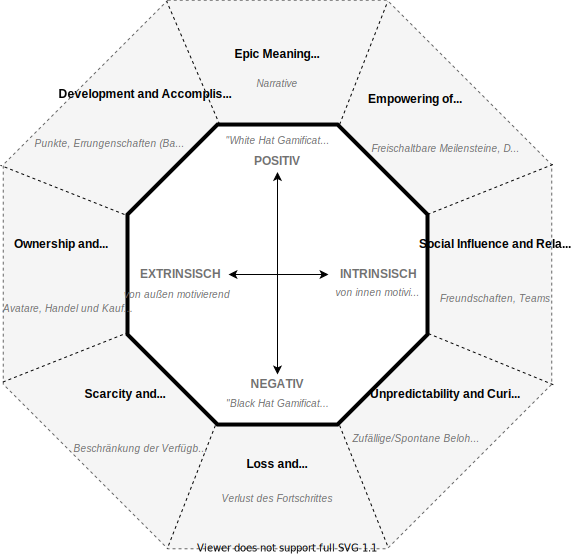
\includegraphics[width=0.75\linewidth, bb=0 0 408 402]{octalysis.pdf}
\caption{Die von Yu-kai Chou entwickelte Gamification-Taxonomie \enquote{Octalysis} als Oktagon mit beispielhaften Gamification-Elementen. Mit freundlicher Genehmigung \cite{chou_actionable_2019}.}\label{fig:octalysis}
\end{figure}

\noindent Weiterhin ordnet Chou diesen Teilzielen die jeweiligen Gamification-Elemente zu. So seien die weit verbreiteten Gamification-Elemente Punkte, Ranglisten und Errungenschaften (bspw. in Form von Badges) zuzuordnen in die Kategorie \enquote{Development and Accomplishment}. Die in \Cref{fig:octalysis} gezeigte Anordnung der acht Teilziele teilt Chou nochmals horizontal und vertikal. Die links in der Abbildung gezeigten Ziele zielten auf die durch äußere Reize hervorrufbare (extrinsische) Motivation des Nutzers ab, während die rechts gezeigten Ziele die von dem Nutzer selbst stammende (intrinsische) Motivation unterstützten. Außerdem seien die weiter oben angebrachten Ziele positiver als die weiter unten gezeigten Ziele, wie zum Beispiel \enquote{Loss and Avoidance}. Diese Teilung illustriert Chou als \enquote{White Hat Gamification} und \enquote{Black Hat Gamification}, was eine Analogie zum legalen White Hat Hacking und zum illegalen Black Hat Hacking darstellt. Eine nach diesen Zielen orientierte Gamification bezeichnet Chou als \enquote{Level 1 Octalysis}. Unter \enquote{Level 2 Octalysis} beschreibt er eine Gamification, welche die genannten Ziele der jeweiligen Phase des Spielers anpasst, wobei der Spieler das Spiel zunächst entdeckt, danach dessen Regeln erlernt und Ziele erreichen möchte und schließlich nach erreichen aller Ziele nach weiteren Motivationen sucht. Zusätzlich ließe sich hieran nach Chou die \enquote{Level 3 Octalysis} anschließen, die diese Faktorisierung der Spielphasen noch zusätzlich um eine Faktorisierung der Spielertypen erweitert.
